\chapter{Resultados Obtidos}

Para validar o sistema é preciso testar os requisitos: mecânicos, de custo, e de desempenho do aplicativo atuando em conjunto com a eletrônica. Então, foram realizados uma sequência de testes em campo. Além disso, a plataforma fora enviada para um astrofotógrafo e Engenheiro, convidado, que conduziu testes usando seu equipamento.\footnote{Relatório do Astrofotógrafo Ricardo Batista pode ser acessado neste link: LINK AQUI} A tabela \ref{} lista todos os testes realizados com o sistema.

\section{Requisitos mecânicos}

Os objetivos mecânicos da plataforma foram alcançados com ressalvas. A plataforma montada totalizou 716g sem o Ball Head da câmera, estando dentro da faixa de peso comparando com dispositivos similares no mercado. Além disso, alguns componentes não se comportaram totalmente como o esperado, no caso da Impressão 3D; e além disso, existe um erro de inconsistência e vibração motivado por falha de fabricação que deve ser analizado.


\subsection{Impressão 3D}
A engrenagem menor é o elo mais fraco no sistema de transmissão, isso se deve pelo seu tamanho mais reduzido. A primeira versão da impressão 3D acabou sofrendo um rachamento por não suportar o torque do motor. Na Figura \ref{fig:engrenagem} é possível verificar que o rasgo se forma perpendicularmente com a tangente da engrenagem, tornando mais evidente o motivo da ruptura.

\begin{figure}[htb]
	\centering
	\caption{Engrenagem com rachamento em evidência}
	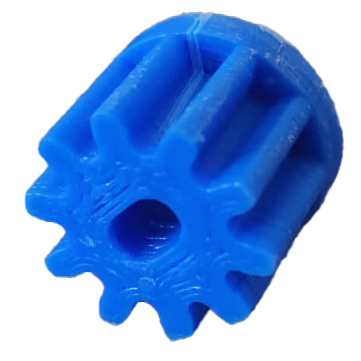
\includegraphics[width=0.25\linewidth]{figuras/resultados/engrenagem}
	\label{fig:engrenagem}
	\fonte{Autor.}
\end{figure}

Ademais, quando a engrenagem apresentou a rachadura, o peso do sistema totalizava mais de 2,5kg com o ball head Maxxi Grua, câmera CANNON 6D MARK II e uma lente 70-200mm. Contudo, este acontecimento não invalida o projeto pois ocorreu com um peso de rastreamento superior à meta proposta, e, por isso, recomenda-se cautela em situações onde o equipamento se aproxima ou ultrapassa a marca de 2,5kg de peso total. A tabela \ref{} discrimina o peso de todos testes realizados com a plataforma -- pelo autor ou pelo convidado--, e o resultado.

 

\subsection{Eixo Curvado}
Além do problema com a engrenagem, o movimento de rotação da plataforma se mostrou inconstante em certos pontos. Essa variação reflete a não idealidade da curvatura do eixo rosqueado. A Figura \ref{fig:validaçãoBarraRoscada} torna claro a discrepância entre como deveria ser, e como ficou. Esse erro de fabricação gerou inconsistência em certos pontos no funcionamento da plataforma, e eles serão demonstrados na próxima seção.

\begin{figure}[htb]
	\centering
	\caption{Erro de fabricação demarcado em vermelho, onde a barra apresenta uma curvatura que varia em relação ao desenho técnico}
	\includegraphics[width=0.8\linewidth]{figuras/resultados/validaçãoBarraRoscada}
	\label{fig:validaçãoBarraRoscada}
	\fonte{Autor.}
\end{figure}


\subsection{Análise de Consistência}
\label{sec:vibracao}

A velocidade e vibração da plataforma foram analisados por meio de um sensor acelerômetro instalado na base superior, alinhado com o eixo rosqueado, como demonstra a Figura \ref{fig:sensorInstaladoPlataforma}. Com esses testes, foi possível comparar diferentes cenários de uso de elementos amortecedores no sistema e o seu impacto na consistência e vibração. Os dados foram obtidos em uma taxa de 100Hz, utilizando um Arduíno e comunicação Serial, com um notebook que armazenava os dados \footnote{O sistema de captação de dados com o sensor está documentado neste repositório do Github: Link AQUI}. 

\begin{figure}[htb]
	\centering
	\caption{Sensor instalado na base superior}
	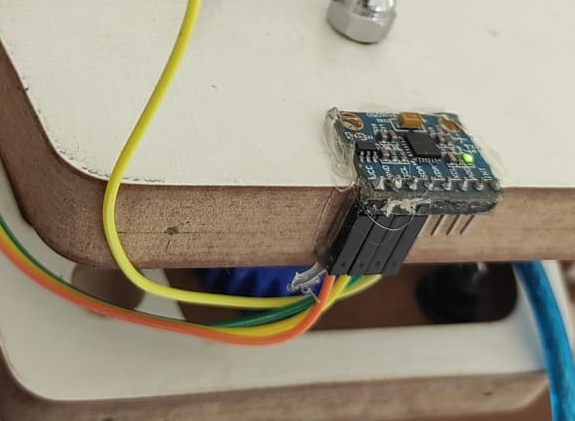
\includegraphics[width=0.35\linewidth]{figuras/resultados/sensorInstaladoPlataforma}
	\label{fig:sensorInstaladoPlataforma}
	\fonte{Autor.}
\end{figure}

Então, os dados obtidos no primeiro teste -- que constam na Figura \ref{} --, demonstram que existia uma inconstância na velocidade angular do sistema, além de um excesso de vibração. Além disso, com os dados da Figura \ref{}, confirmou-se que existe a necessidade de elementos para dissipar a vibração. Ressalta-se ainda que existem pontos de intensificação da vibração, e, pelo período temporal onde acontece, é possível inferir que são decorrentes do erro de fabricação do eixo curvado. 

\begin{figure}[!htb]
	\centering
	\caption{Primeiro teste do sistema}
	\includegraphics[width=0.9\linewidth]{figuras/resultados/antes}
	\label{fig:antes}
	\fonte{Autor.}
\end{figure}

\begin{figure}[!htb]
	\centering
	\caption{Teste do sistema com}
	\includegraphics[width=0.9\linewidth]{figuras/resultados/depois}
	\label{fig:depois}
	\fonte{Autor.}
\end{figure}

\section{Custo total do sistema}
O custo dos materiais e processos de fabricação estão descritos na tabela \ref{table:custo}\footnote{Alguns valores são aproximados pois foram doados pela Universidade}, com a qual pode se constar um total de x reais envolvendo materiais e fabricação de componentes. Comparando ao valor do NyxTech -- que possui uma construção e materiais similares, com um preço de US\$ 110 -- o EasyTracker conseguiu vencer a meta de custo.  

\begin{table}[!htb]
	\centering
	\caption{Descrição aproximada dos Custos do Sistema}
	\begin{tabular}{c|c}
	Item	&	Custo	\\\hline\hline
	MDF	15mm	&	R\$ 25,00		\\\hline
	Corte a Laser			&	R\$ 100,00		\\\hline
	PCB			&	R\$ 50,00		\\\hline
	Componentes Eletrônicos			&	R\$ 95,00		\\\hline
	Outros Materiais		&	R\$ 35,00		\\\hline\hline
	Total			&	R\$ 305,00		\\
	\end{tabular}
	\label{table:custo}
	\fonte{Autor.}
\end{table}


\section{Análise de desempenho do aplicativo}
O Software pode ser avaliado com relação ao uso e implementação das heurísticas de desenvolvimento, com relação ao desempenho em hardware -- consumo de processamento e memória --, e ainda pode ser avaliada com Feedbacks dos usuários. 

\subsection{Interface Gráfica}
Quando à interface e recursos, é possível avaliar de forma qualitativa como as 10 Heurísticas de Nielsen foram utilizadas. Os status cruciais para funcionamento são todos visíveis: o status \textit{bluetooth} do sistema é visível por meio do estado do botão de conexão na tela de visualização do perfil. Nas telas de alinhamento, se o sistema está alinhado, os ícones ficam esverdeados, caso contrário ficam avermelhados.

Além disso, as cores e os elementos de ícones são similares com o que os usuários estão acostumados, como os ícones nas telas de perfis de localização que fazem sentido para o contexto e são minimalistas. Além disso, as telas de alinhamento se assemelha a uma bolha de nível onde o acelerômetro é empregado. Na tela de alinhamento com o polo magnético, o sistema emula uma bússola. 

Nessas mesmas telas de alinhamento, os usuários podem controlar livremente o fluxo das telas de alinhamento. Dessa forma conseguem conferir alguma informação que possam ter deixado passar, assim como podem navegar para telas de ajudas e retornar.

Não obstante, a consistência desses padrões nas telas de alinhamento também foram consolidado nas telas de perfis. As ações de criar, editar, e visualizar um perfil usam por base a mesma tela, facilitando para o usuário entender o que ocorre no sistema. 

Além disso, a prevenção de erros é feita de forma ativa relembrando o usuário de, por exemplo, recomendando uma calibração da bússola ao entrar na tela de alinhamento azimutal, ou também com um popup para atualizar os dados de declinação magnética em localizações que foram armazenadas a mais e 2 meses. A prevenção também ocorre nas entradas de dados:  onde o usuário precisa inserir valores de latitude e declinação, que devem ser valores decimais (Figura \ref{fig:gpsedit}). No entanto, eles podem ser escritos em graus, minutos e segundos, mas o usuário não vai conseguir inserir dessa forma, pois, o teclado numérico não permite essa formatação.

\begin{figure}[!htb]
	\centering
	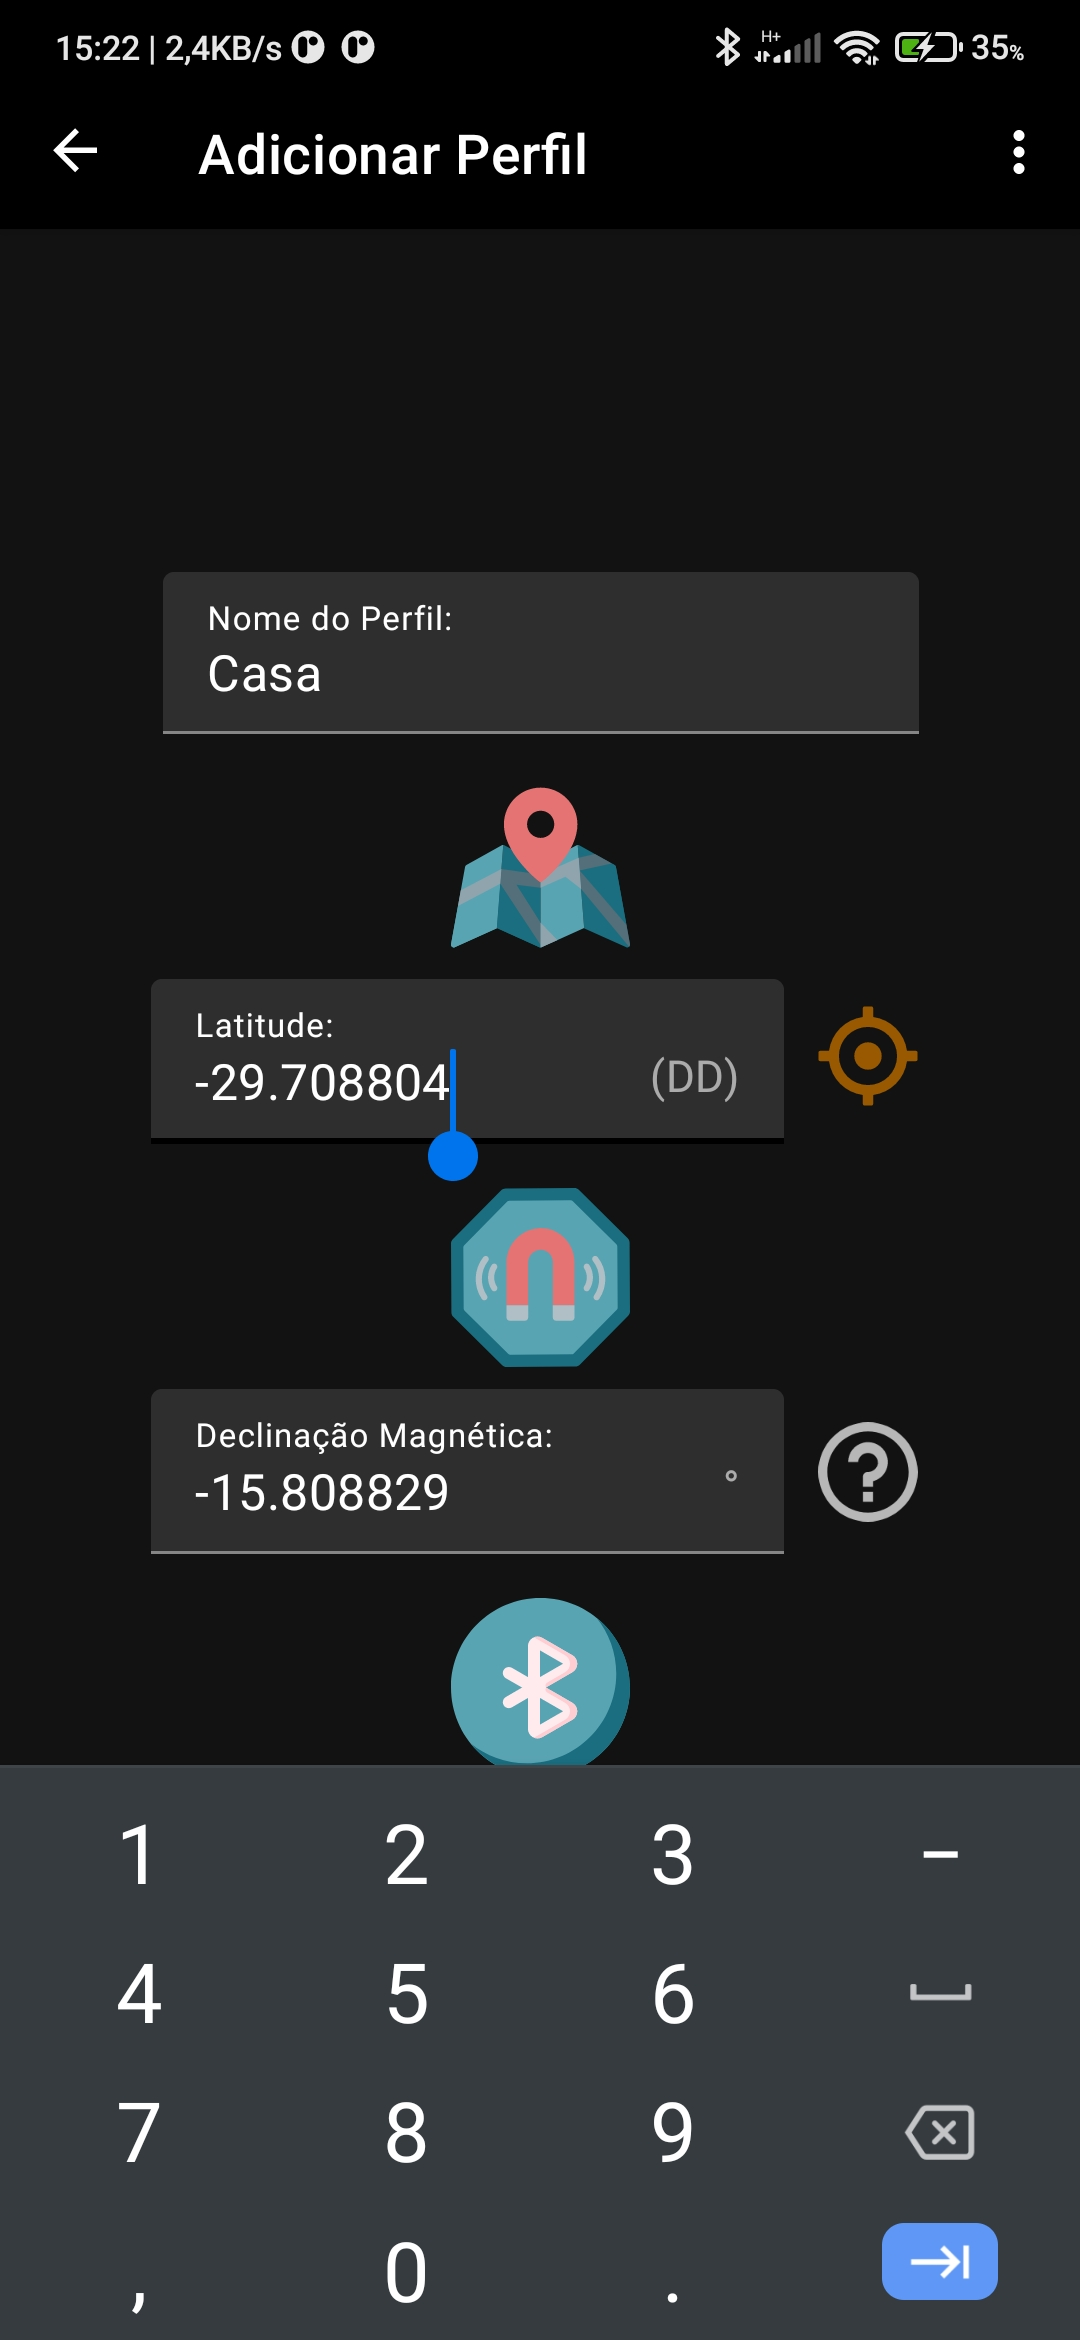
\includegraphics[width=0.3\linewidth]{figuras/resultados/gpsedit}
	\caption{Teclado só permite uso de vírgula e ponto, não permitindo aspas e sinal de grau $ (^\circ) $}
	\label{fig:gpsedit}
\end{figure} 

Dessa forma, o desenvolvimento da interface gráfica do aplicativo conseguiu atingir um estágio de desenvolvimento compatível com o estado da arte atual relativo a criação de aplicativos Android ou outros Softwares. As heurísticas foram respeitadas e a implementação é fluída, os itens estão dispostos respeitando uma hierarquia visual que está em conluio com a identidade do projeto e os recursos do Sistema Android. 

\subsection{Desempenho}
O aplicativo foi lançado na loja de aplicativos Android via Google Play Console. O Console de desenvolvedor realiza testes automáticos com alguns dispositivos e avalia o desempenho. Os resultados indicam que o aplicativo pode ter problemas de lentidão em hardwares mais antigos e com menor capacidade de memória e armazenamento; mas, ao mesmo tempo, não detectou nenhum problema em sistemas mais recentes (Figura \ref{fig:relatorioDesempenho}).

\begin{figure}[htb]
	\centering
	\caption{Resultados apresentados no Google Play Console}
	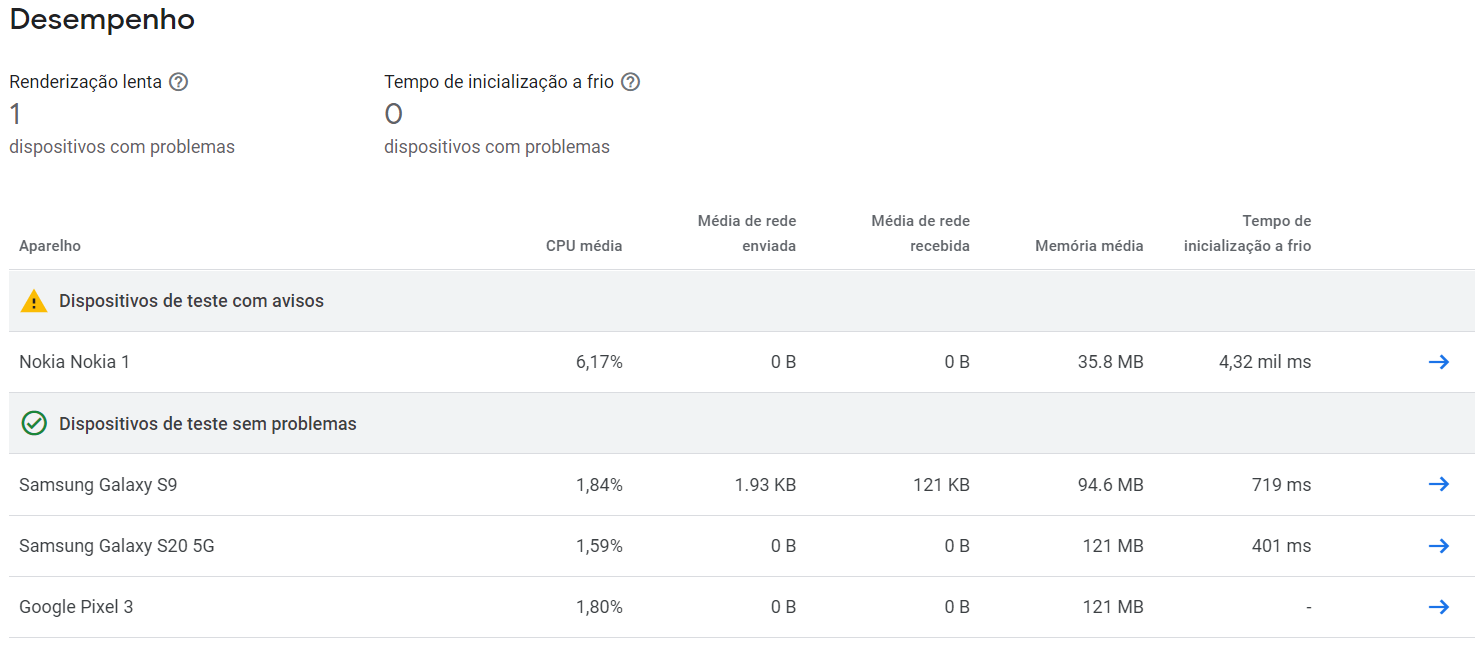
\includegraphics[width=\linewidth]{figuras/resultados/relatorioDesempenho}
	\label{fig:relatorioDesempenho}
	\fonte{Autor.}
\end{figure}

Considerando que o dispositivo com dificuldade no processamento é bem defasado, é razoável considerar que o aplicativo não será um problema para a grande maioria dos dispositivos, principalmente os mais recentes. 

\section{Comparativo Geral}
Os 3 pontos avaliados anteriormente listam eventuais problemas que afetaram a consistência do sistema e projeto como um todo. No entanto, é necessário verificar ainda se, apesar desses entraves, o projeto consegue cumprir com os objetivos gerais.

Dessa forma, é preciso avaliar se o método de alinhamento consegue ser tão confiável quanto os métodos tradicionais de luneta e laser, assim como se as especificações de erro estão dentro da margem comercial. Assim, dois erros podem ser avaliados: o erro inerente ao sistema mecânico, nomeado de erro periódico; e o erro relativo ao processo de alinhamento.


\subsection{Erro Periódico}

O erro periódico mensura a oscilação do sistema de transmissão, gerada por variações na montagem e encaixe dos componentes. O período desse erro é definido pelo tempo total levado para que o motor de passo realize 1 rotação. O erro é medido em arc segundos, que é uma unidade que irá avaliar o quanto uma estrela oscilou sua posição pelo visor da câmera, independente da lente utilizada. O teste que mensura esse erro é realizado apontando a câmera para qualquer alvo no céu, desalinhando o rastreador propositalmente, e realizando uma fotografia de longa exposição. 

Então, apontou-se a câmera para Júpiter, utilizando a Câmera DSC-HX300, com comprimento focal em 192mm, e assim fora possível extrair a seguinte oscilação do posicionamento da estrela ao longo de 8 fotografias captadas em intervalos de 8s. Empilhando as imagens, têm-se o resultado da Figura \ref{fig:periodicErrorImage}. Usando um software editor de imagens, é possível desenhar sobre esses pontos uma forma de onda. O erro periódico é igual a distância de pico a pico medida em arc segundos. Essa distância é medida inicialmente em pixel, e posteriormente convertida para arcsec com a equação (\ref{eq:arc}), sabendo que essa câmera tem um tamanho de pixel ($ px_s $) igual a  $ 1,19~um $ . Nos testes realizados, a média de erro foi igual  $ 63~arcsec  $


\begin{equation}
	angResolution = \dfrac{px_s (\mu m) * 206,3}{d (mm)}
	\label{eq:arc}
\end{equation}

\begin{figure}[htb]
	\centering
	\caption{Pontos obtidos com as 8 imagens empilhadas ao longo de 80s}
	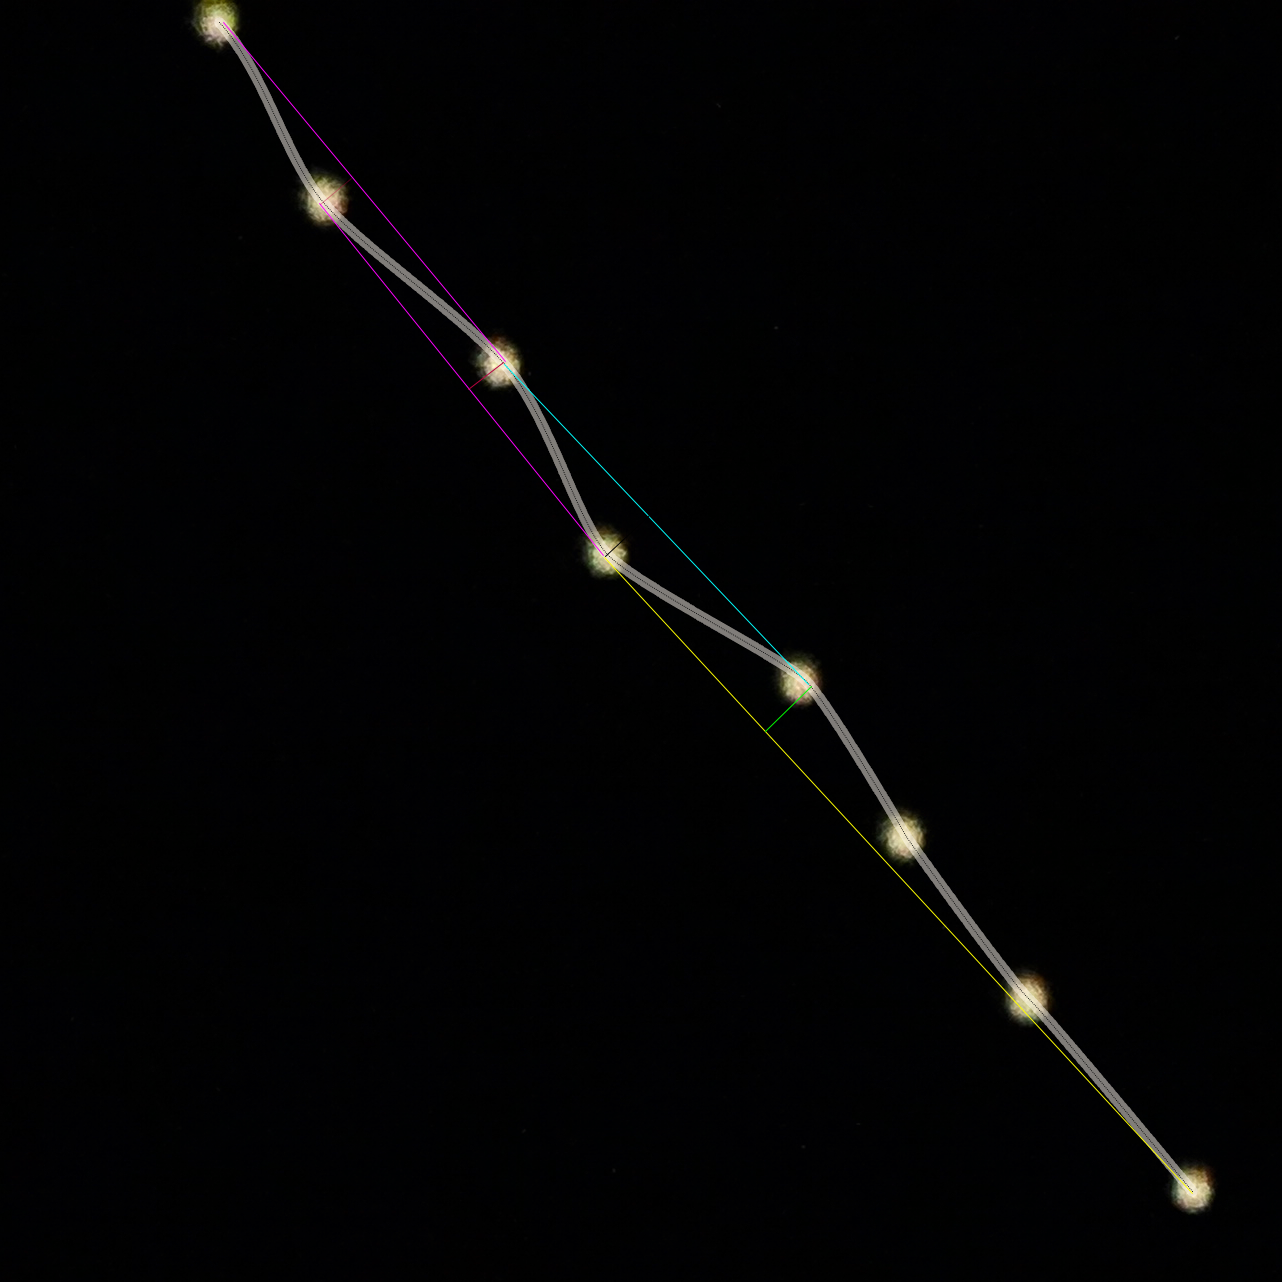
\includegraphics[width=.5\linewidth]{figuras/resultados/periodicErrorImage}
	\label{fig:periodicErrorImage}
	\fonte{Autor.}
\end{figure}


\subsection{Erro de Alinhamento}

Como o principal objetivo do rastreamento é o aumento do tempo de rastreamento, buscou-se determinar uma regra de cálculo -- no mesmo formato das regras dos 300 ou 500 -- de tempo de exposição adequado para o EasyTracker. De forma similar, o NyxTech -- (figura \ref{fig:nyxtracker}) já apresentado anteriormente --, possui a sua regra dos XXX com alinhamento laser e XXX com alinhamento via luneta \cite{}.

Para determinar o valor da regra, o alinhamento foi realizado para um conjunto de diferentes lentes, e verificou-se qual tempo máximo de exposição para que não houvesse rastro significativo na imagem. 

%todo: terminar
